\documentclass{standalone}
\usepackage{tikz}
\usetikzlibrary{arrows.meta,calc}
\def\iangle{15} % Angle of the inclined plane
\def\down{-90}
\def\arcr{1.5cm} % Radius of the arc used to indicate angles
\def\boxsize{1cm}
\def\slopelength{6cm}
\def\axlength{1.25cm}
\def\boxgrav{1cm}
\def\trianglegrav{1.2cm}
\def\angle{180 - \iangle}
\begin{document}
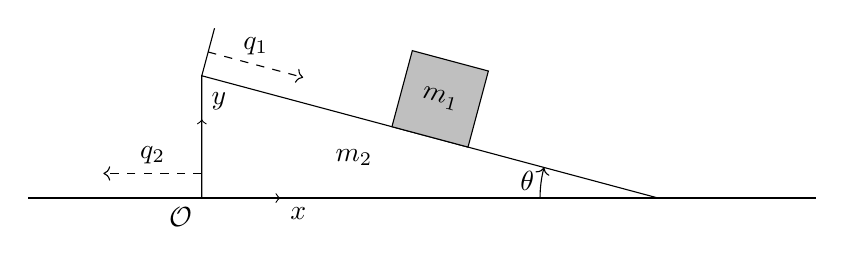
\begin{tikzpicture}[
	M/.style={rectangle,draw,fill=lightgray,minimum size=\boxsize,thin},
	axis/.style={->,dashed},
	force/.style={->,>=latex}
	]
	\draw (0,0) coordinate (base) -- coordinate[pos = .5] (mid) ++ (\angle:\slopelength) coordinate (origin) -- ++ (0,-{\slopelength*sin(\iangle)})-- cycle;
	
	\draw (origin) -- coordinate[pos = .5] (q1axis) ++ (\angle - 90:{\axlength/2});
	\draw[axis] (q1axis) -- node[above] {$q_1$} ++ (-\iangle:\axlength);
	
	\draw (base) --  ++ ({\slopelength*cos(\angle)},0) -- coordinate[pos = .5] (q2axis) ++ (0,{\axlength/2});
	\draw[axis] (q2axis) -- node[above] {$q_2$} ++ (-\axlength,0);
	
	
	\draw (2,0) -- (0,0) -- ++ (-\slopelength,0) -- ++ (-2,0);
	
	\draw[->] (base)++(-\arcr,0) arc (0:-\iangle:-\arcr);
	\path (base)++(-\iangle*.5:-\arcr-5pt) node {$\theta$};
	\draw (base) -- ++(180:\arcr);
	
	\coordinate (triangle) at (-{2*cos(\iangle)*\slopelength/3},{sin(\iangle)*\slopelength/3});
	
	\draw (mid) node[M, rotate= - \iangle, yshift = \boxsize/2] (M) {\(m_1\)};
	\node at ($(origin) - ({\slopelength*cos(\angle)/3},{2*\slopelength*sin(\iangle)/3})$) {\(m_2\)};
	
	\draw[-to] ($(1,0)!(q2axis)!(0,0)$) -- ++(0,1) node[anchor = south west] {\(y\)};
	\draw[-to] ($(1,0)!(q2axis)!(0,0)$) -- ++(1,0) node[anchor = north west] {\(x\)};
	\node[anchor = north east] at ($(1,0)!(q2axis)!(0,0)$) {\(\mathcal{O}\)};
\end{tikzpicture}
\end{document}